\documentclass{article}
\usepackage{styles/project_style} % Assuming you have this style file
\addbibresource{references/projects.bib}

% --- TITLE PAGE INFORMATION ---
\title{Introduction to the Allee effects}

\begin{document}
\maketitle

\section{What is the Allee Effect?}
Imagine a small group of animals colonizing a new island, or a patch of rare plants reduced to just a few individuals. Common sense might suggest that with abundant resources and little competition, their population should grow rapidly. However, sometimes the opposite happens: small populations struggle to survive or reproduce, and their growth rate actually \emph{increases} as the population becomes slightly larger or denser.

This counter-intuitive phenomenon is known as the \textbf{Allee Effect}, named after the ecologist Warder Clyde Allee who extensively studied social aggregation and cooperation in animals. It describes a situation in population ecology where, at \emph{low} population sizes or densities, there is a \textbf{positive relationship} between the population size (or density) and the \emph{per capita} (average individual) growth rate. In simpler terms, individuals in very small or sparse populations sometimes do worse in terms of survival and reproduction than individuals in slightly larger or denser populations.

\begin{figure}[htbp]
  \centering
  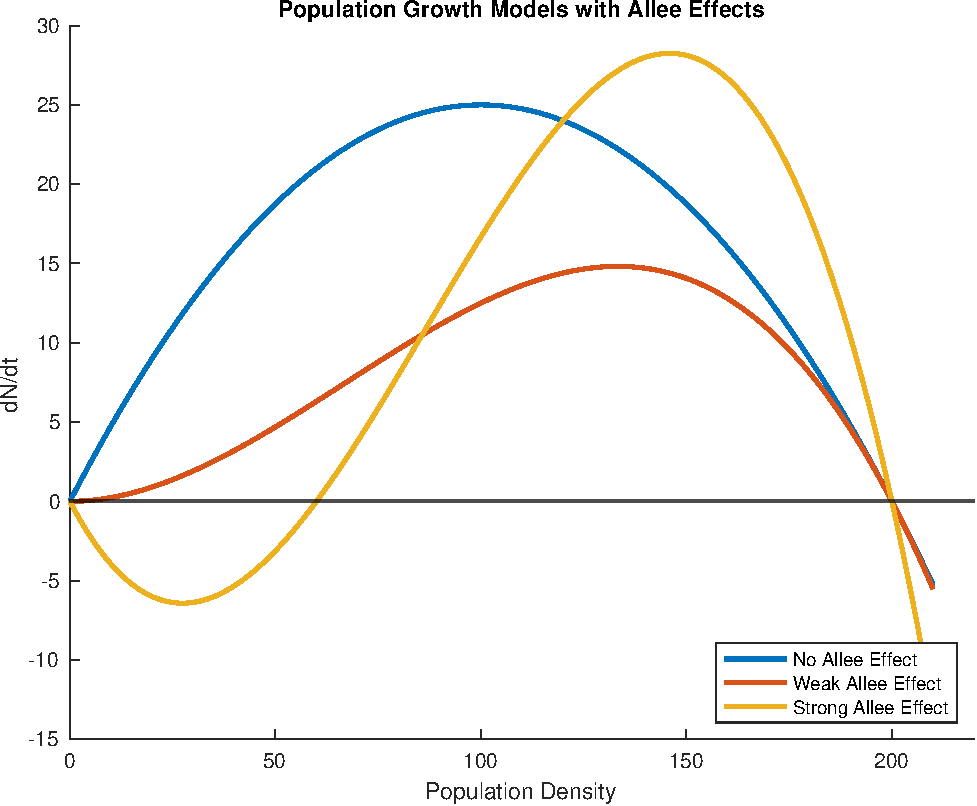
\includegraphics[width=0.55\textwidth]{projects/allee_effect/images/allee_effects.pdf}
  \caption{Illustration of the Allee effects in population dynamics. Curves shows no Allee effect (logistic growth), weak and strong Allee effect. Y-axis show population growth, while x signifies population density.}
  \label{fig:allee-effects}
\end{figure}

This contrasts  with the more familiar concept of density-dependent limitation (like in the logistic model), where growth rates \emph{decrease} as population density increases due to factors like competition for resources, increased disease transmission, or predation. The Allee effect focuses specifically on the challenges faced at the \emph{lower end} of the population size spectrum.

The Allee effect arises from mechanisms that require or benefit from a certain number of individuals being present. Key components contributing to the Allee effect include:
\begin{itemize}
    \item \textbf{Mate finding difficulty:} Individuals in sparse populations may struggle to find compatible mates.
    \item \textbf{Reduced cooperative defense:} Small groups may be less effective at deterring predators compared to larger groups.
    \item \textbf{Reduced cooperative feeding:} Some species rely on group hunting or foraging strategies that become inefficient at low numbers.
    \item \textbf{Environmental conditioning:} Some organisms (like certain plants or microbes) modify their environment in ways that benefit the group, an effect diminished in small populations.
    \item \textbf{Social thermoregulation:} Animals that huddle for warmth may suffer in small groups.
    \item \textbf{Reduced pollination/fertilization success:} For plants or sessile marine invertebrates.
    \item \textbf{Inbreeding depression and loss of genetic diversity:} More pronounced in very small populations.
\end{itemize}

Understanding the Allee effect is crucial because it implies that populations can have a \textbf{minimum viable size} or density. If a population drops below this threshold, its growth rate can become negative, leading it towards extinction even if resources are theoretically plentiful.

\section{Types of Allee Effects}

Ecologists distinguish between two main types:

\begin{itemize}
    \item \textbf{Strong Allee Effect:} Characterized by a critical population threshold size or density ($A$). Below this threshold ($N < A$), the \emph{per capita} population growth rate becomes negative ($\frac{1}{N}\frac{dN}{dt} < 0$), meaning the population is destined to decline towards extinction unless boosted by immigration or other factors.
    \item \textbf{Weak Allee Effect:} The \emph{per capita} population growth rate is still positive at low densities, but it is lower than it would be at slightly higher densities. There is no critical extinction threshold, but the population grows more slowly when small compared to intermediate sizes.
\end{itemize}

\section{Why is the Allee Effect Important?}

Recognizing and understanding the Allee effect has significant implications:

\begin{itemize}
    \item \textbf{Conservation Biology:} It helps explain why small, fragmented populations are particularly vulnerable to extinction and highlights the need to maintain populations above critical thresholds. Recovery plans may need to focus on increasing population size or density directly.
    \item \textbf{Invasion Biology:} It can explain why some introduced species fail to establish despite suitable conditions – they may arrive in numbers too small to overcome Allee effects (e.g., finding mates).
    \item \textbf{Pest Management:} For pests exhibiting Allee effects, control strategies that drive the population below the critical threshold ($A$) can be particularly effective, leading to eradication rather than just suppression.
    \item \textbf{Resource Management:} In fisheries or wildlife harvesting, Allee effects mean that over-harvesting can push a population below a recovery threshold, making sustainable management more complex.
    \item \textbf{Ecological Theory:} It adds crucial realism to population models, demonstrating that growth is not always maximal at the lowest densities.
\end{itemize}

\section{Mathematical Representation}

The Allee effect can be incorporated into population growth models by modifying the per capita growth rate term. There is no single mathematical representation of the Allee effect; instead, several alternative formulations are used depending on whether the goal is to model strong vs. weak effects, the presence of thresholds, or to provide flexible fitting to empirical data.

\paragraph{Logistic Growth Model:}
For comparison, the continuous logistic model is written as:
\[
\frac{dN}{dt} = rN\left(1 - \frac{N}{K}\right)
\]
Here, $N$ is population size, $t$ is time, $r$ is the intrinsic growth rate, and $K$ is the carrying capacity. The per capita growth rate is highest when $N$ is very small and declines linearly as $N \to K$.

\paragraph{Modeling a Weak Allee Effect:}
A simple way to model reduced growth at low population sizes (without an extinction threshold) is:
\[
\frac{dN}{dt} = \frac{r}{K}N^2\left(1 - \frac{N}{K} \right)
\]
This represents a \textbf{weak Allee effect}, where the growth rate is low when $N$ is small, but still positive. The $N^2$ term ensures slow growth when the population is small.

\paragraph{Modeling a Strong Allee Effect:}
To introduce a critical population threshold (below which the population declines), one common form is:
\[
\frac{dN}{dt} = rN\left(\frac{N}{A} - 1\right)\left(1 - \frac{N}{K}\right)
\]
Here, $A$ is the Allee threshold:
\begin{itemize}
    \item If $N < A$, growth is negative (extinction risk).
    \item If $A < N < K$, population increases.
    \item If $N > K$, population declines due to overpopulation.
\end{itemize}
The per capita growth rate:
\[
\frac{1}{N}\frac{dN}{dt} = r\left(\frac{N}{A} - 1\right)\left(1 - \frac{N}{K}\right)
\]
is negative at low and high densities, positive only in between.

\paragraph{Flexible Models:}
More general forms, such as those proposed by Boukal \& Berec (2002), allow flexible interpolation between weak and strong Allee effects:
\[
\frac{dN}{dt} = rN\left(1 - \frac{N}{K} \right)\left( \frac{N - A}{K} \right)
\]
Here, the parameter $A$ determines the nature of the Allee effect:
\begin{itemize}
    \item $A < 0$: No Allee effect.
    \item $A = 0$: Logistic growth.
    \item $A > 0$: Strong Allee effect.
\end{itemize}

These various formulations emphasize that the Allee effect is a concept rather than a single equation—different biological processes and assumptions lead to different mathematical expressions.


\section{MATLAB Implementation of Population Growth Models}

The following MATLAB script computes and plots three population‐growth curves:
\begin{itemize}
  \item \textbf{Logistic growth} (no Allee effect),
  \item \textbf{Weak Allee effect}, using a quadratic term that slows growth at low densities but never yields negative growth,
  \item \textbf{Strong Allee effect}, adding a threshold \(A_\text{strong}\) below which growth becomes negative.
\end{itemize}

In the original code, both “growth\_weak” and “growth\_strong” used the threshold form 
\(\displaystyle rN(1 - N/K)(N/A - 1)\), so “weak” was in fact just a strong effect with a smaller \(A\).  
Below, the weak effect is corrected to the common quadratic form
\(\displaystyle \tfrac{r}{K}N^2(1 - N/K)\).

\subsection{Model Definitions}
\begin{itemize}
  \item \(\displaystyle\frac{dN}{dt} = r\,N\bigl(1 - \tfrac{N}{K}\bigr)\)  
        — logistic, no Allee effect.
  \item \(\displaystyle\frac{dN}{dt} = \frac{r}{K}\,N^2\bigl(1 - \tfrac{N}{K}\bigr)\)  
        — weak Allee effect, growth reduced at low \(N\) but always non‐negative.
  \item \(\displaystyle\frac{dN}{dt} = r\,N\bigl(\tfrac{N}{A_\text{strong}} - 1\bigr)\bigl(1 - \tfrac{N}{K}\bigr)\)  
        — strong Allee effect, negative growth for \(N < A_\text{strong}\).
\end{itemize}

\subsection{MATLAB Code}
\begin{lstlisting}[caption={Analyze simulation results (Calculation part)}]
%--- Model parameters and density vector
r = 0.5;       % Intrinsic growth rate
K = 200;       % Carrying capacity
A_strong = 60; % Strong effect threshold
N = linspace(0, K*1.05, 5000);

%--- Compute growth curves
growth_no = r * N .* (1 - N/K);
growth_weak = (r/K) * N.^2 .* (1 - N/K);
growth_strong = r * N .* (1 - N/K) .* (N/A_strong - 1);

%--- Plot all three curves
figure;
hold on
    plot(N, growth_no, 'LineWidth', 2);
    plot(N, growth_weak, 'LineWidth', 2);
    plot(N, growth_strong, 'LineWidth', 2);
    yline(0, 'k-', 'LineWidth', 1.5); 
    title('Population Growth Models with Allee Effects');
    xlabel('Population Density'); ylabel('dN/dt');
    legend('No Allee Effect',  'Weak Allee Effect',
            'Strong Allee Effect', 
            'Location', 'southeast');
    xlim([0, K*1.1])
hold off
\end{lstlisting}

\paragraph{Explanation}
\begin{itemize}
  \item \textbf{Logistic}: growth is maximal at \(N\!\to\!0\) and declines linearly to zero at \(N=K\).
  \item \textbf{Weak Allee}: the \(N^2\) term makes per‐capita growth low when \(N\) is small, but always non‐negative; no extinction threshold.
  \item \textbf{Strong Allee}: the extra factor \((N/A_\text{strong}-1)\) creates a critical density \(A_\text{strong}\). Below it, \(\tfrac{dN}{dt}<0\) and the population declines.
\end{itemize}



\section{Example Scenario}

Consider a species of colonial seabird that nests in dense groups for protection against gulls.
\begin{itemize}
    \item \textbf{Very Low Density (Below $A$):} If only a few pairs try to nest, they are easily spotted and preyed upon by gulls. Nesting success (offspring produced per pair) is very low, potentially zero or negative net growth. Mate finding might also be harder if individuals are spread out. This population is likely to decline.
    \item \textbf{Intermediate Density (Between $A$ and $K$):} As more pairs join the colony, they benefit from communal defense ("safety in numbers"). More eyes spot predators, and collective mobbing can drive gulls away. Nesting success increases significantly. The population grows.
    \item \textbf{High Density (Approaching $K$):} As the colony becomes very crowded, competition for the best nesting sites increases, disease might spread more easily, and local food resources might become depleted. Nesting success starts to decline again due to these density-dependent limitations. Growth slows and eventually stops or becomes negative if $K$ is exceeded.
\end{itemize}
This scenario illustrates how the per capita success rate (and thus growth rate) can be lowest at very low densities (the Allee effect) before declining again at very high densities (resource limitation).

\section{Literature}
\subsection{General introduction}
The topic is well discussed in several online resources. Wikipedia is a good starting point. There are many videos on YouTube on the topic. See:
\begin{itemize}
    \item \textcite{WikiAlleeEffect2025}
    \item \textcite{Drake2011_allee}
    \item \textcite{Kramer2017}
\end{itemize}
\subsection{Journal Club}
Allee effect is extensively used in population modeling. Here are several papers that can be discussed in the Journal Club presentation.
\begin{itemize}
    \item \textcite{Mumby2024_allee} 
    \item \textcite{Fadai2020_allee}
    \item \textcite{Tobin2011_allee}
\end{itemize}


\section{Conclusion}

The Allee effect describes the crucial concept that "more" is not always "worse" in population dynamics; sometimes, especially at low numbers, "more is better." It highlights the importance of social interactions, cooperation, and demographic thresholds for population persistence and growth. Recognizing Allee effects is vital for effective conservation strategies, understanding biological invasions, and managing harvested populations, adding a critical layer of complexity and realism beyond simpler models like basic exponential or logistic growth. Its presence can dramatically alter predictions about population viability and recovery potential.


\printbibliography

\end{document}